{\let\thefootnote\relax\footnotetext{Publication Details: Zhu, F., Emile-Geay, J., McKay, N. P., Hakim, G. J., Khider, D., Ault, T. R., Steig, E. J., Dee, S., \& Kirchner, J. (2019). Climate models can correctly simulate the continuum of global-average temperature variability. Proceedings of the National Academy of Sciences, 201809959. \url{https://doi.org/10.1073/pnas.1809959116}}}

\section{Introduction}
\blindtext

\blindtext

\blindtext

\blindtext

\blindtext

\section{Example figures}
Figure \ref{fig:01} is borrowed from \citet{zhu_climate_2019}.

\begin{figure}[htbp]
\begin{center}
    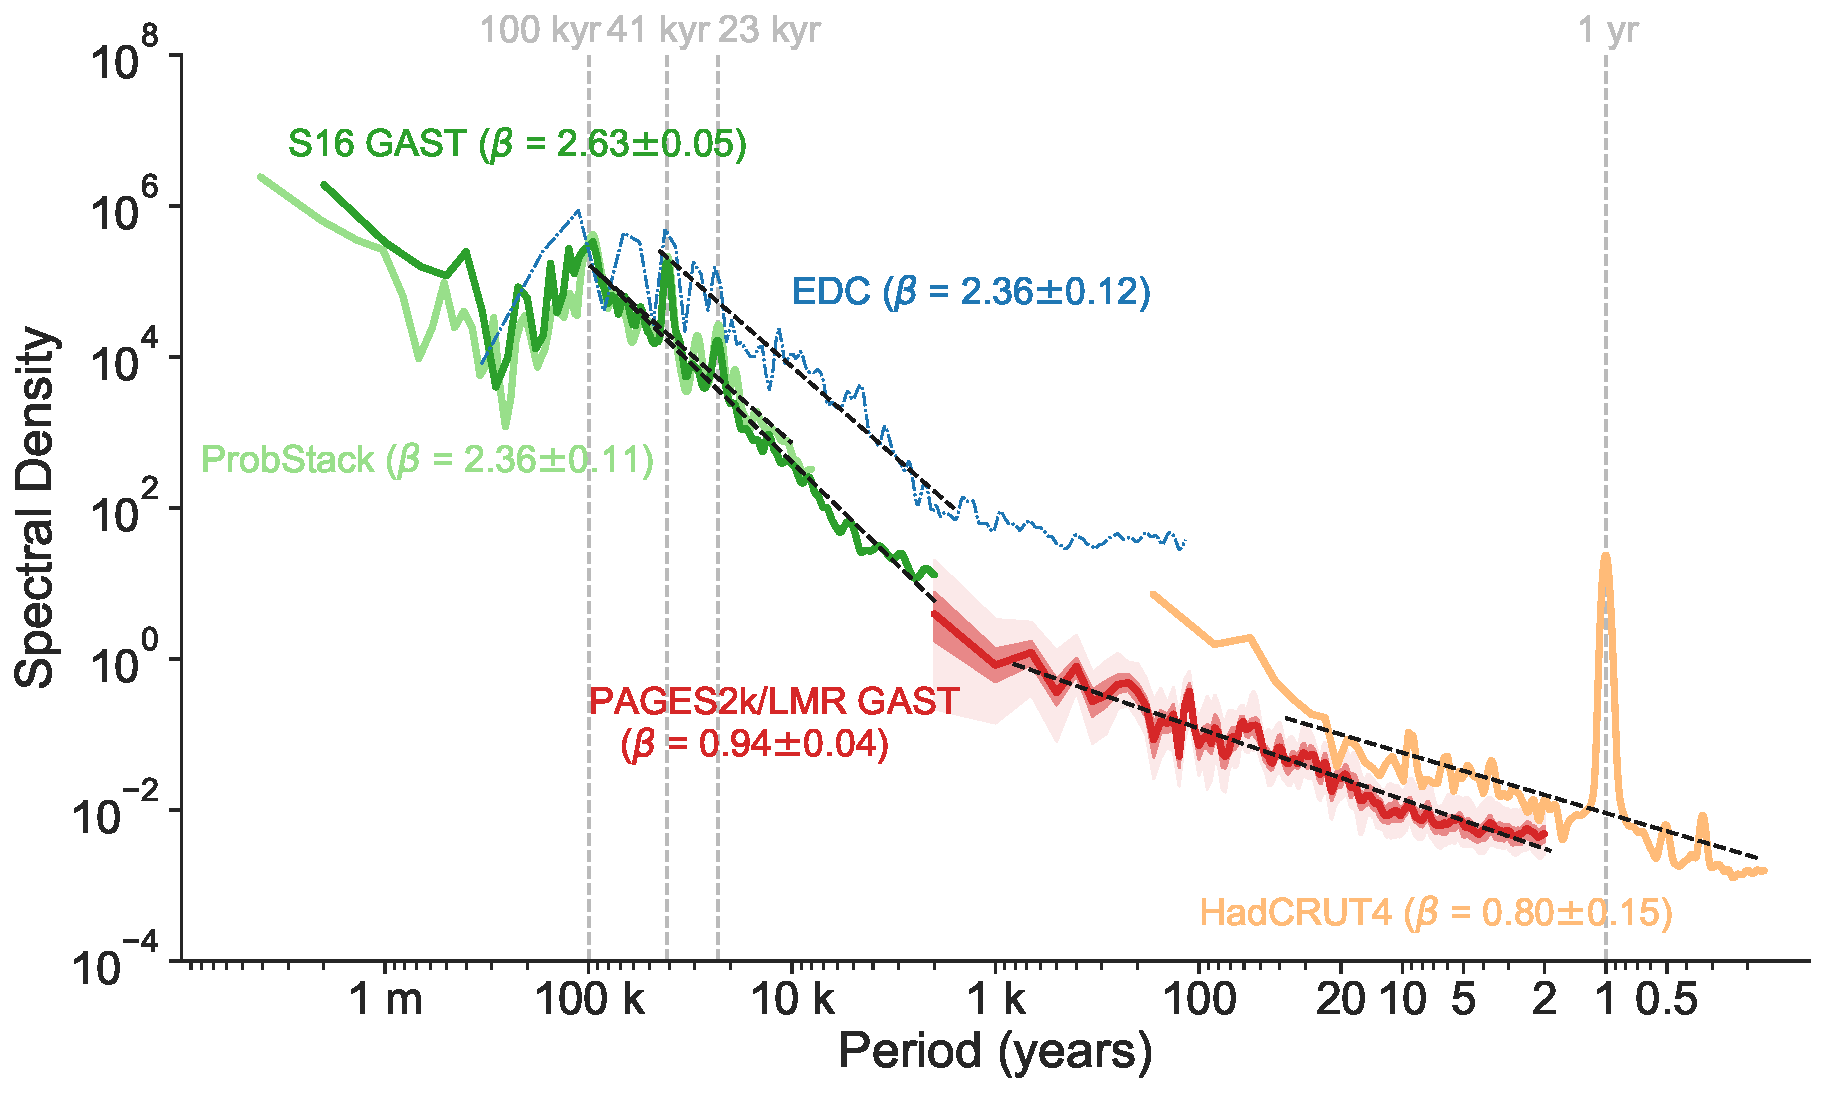
\includegraphics[width=1.0\textwidth,angle=00]{./figs/study-i-01.pdf}
    \caption{Figure borrowed from \citet{zhu_climate_2019}.}\label{fig:01}
\end{center}
\end{figure}


\section{Example tables}
Table \ref{tab:01} is an example of a simple tabular.

\begin{table}[htbp]
\centering
    \caption{Caption text.}\label{tab:01}
%     \begin{adjustbox}{width=\columnwidth,center}  % turn on if the table is too wide
    \begin{tabular}{llll}
        \toprule
        header-01 & header-02 & header-03 & header-04 \\
        \midrule
        column-01 & column-02 & column-03 & column-04 \\
    	\bottomrule
    \end{tabular}
%     \end{adjustbox}
\end{table}

\section{Example equations}
Equation \eqref{eq:01} shows a matrix.

\begin{align}
\bm{S} = \begin{bmatrix}
    \langle \bm{\Psi}_0 \mid \bm{\Psi}_0 \rangle &  \langle \bm{\Psi}_0 \mid \bm{\Psi}_1 \rangle &  \langle \bm{\Psi}_0 \mid \bm{\Psi}_2 \rangle \\
    \langle \bm{\Psi}_1 \mid \bm{\Psi}_0 \rangle &  \langle \bm{\Psi}_1 \mid \bm{\Psi}_1 \rangle &  \langle \bm{\Psi}_1 \mid \bm{\Psi}_2 \rangle \\
    \langle \bm{\Psi}_2 \mid \bm{\Psi}_0 \rangle &  \langle \bm{\Psi}_2 \mid \bm{\Psi}_1 \rangle &  \langle \bm{\Psi}_2 \mid \bm{\Psi}_2 \rangle \\
\end{bmatrix}\label{eq:01}
\end{align}

\section{Conclusion}
\blindtext